%%
%% This is file `apxone.tex',
%% generated with the docstrip utility.
%%
%% The original source files were:
%%
%% ths.dtx  (with options: `apxmin,addfig')
%% 
%% IMPORTANT NOTICE:
%% 
%% For the copyright see the source file.
%% 
%% Any modified versions of this file must be renamed
%% with new filenames distinct from apxone.tex.
%% 
%% For distribution of the original source see the terms
%% for copying and modification in the file ths.dtx.
%% 
%% This generated file may be distributed as long as the
%% original source files, as listed above, are part of the
%% same distribution. (The sources need not necessarily be
%% in the same archive or directory.)


 %% ... sample chapter ...

\section{A First-LEVEL Appendix HEADING}
\lipsum[7-9]

\subsection{A Second-Level Appendix Heading}
\lipsum[10]
\subsubsection{A Third-Level Appendix Heading with a Very Long and
  Complicated Title to Once Again Verify the Formatting}
\lipsum[10-12]
\subsubsection{Another Third-Level Appendix Heading}
\lipsum[10-12]
\paragraph{A fourth-level appendix heading with a long and complicated title
to once again verify the formatting}
\lipsum[13-15]

\subsection{Another Second-Level Appendix Heading but with a
Very Long and Complicated Title to Verify the Formatting}
\lipsum[13-15]

\section{Discussion Using a First-Level Appendix Heading
  Which is Really Long So That It Produces a Two-Line
  Toc Entry}
\lipsum[10-12]

\section{Content with Figures}
\lipsum[10]

\subsection{Floats with Figures}

\lipsum[12-13]

\subsubsection{Simple figure with label}

\lipsum[11]

Add a simple figure, Figure~\ref{fig:fig00}, to illustrate
an entry in the list of figures. %
\begin{figure}[tb]
  \begin{center}
   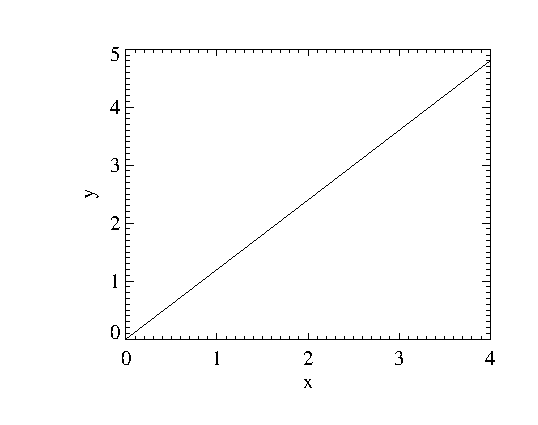
\includegraphics[width=3.75in]{simple.eps}
  \end{center}
  \caption{The caption of the figure.}
\label{fig:fig00}
\end{figure}%
\lipsum[12]

\subsubsection{Figure with psfrag replacement}

\lipsum[13].  Figure~\ref{fig:fig01} illustrates the use
of the psfrag package to place \LaTeX\ math in a graphic.%
\begin{figure}[tb]
  \psfrag{x}{$x$}
  \psfrag{y}{$y$}
  \begin{center}
   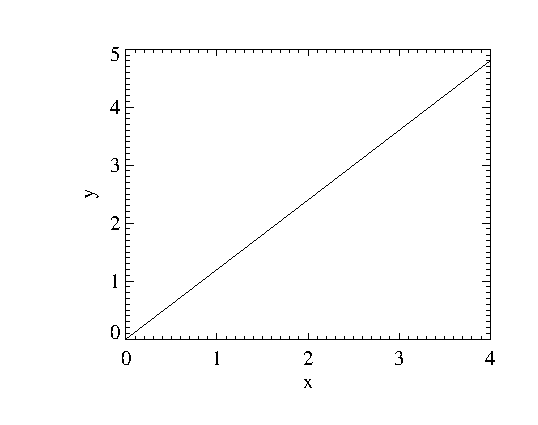
\includegraphics[width=3.75in]{simple.eps}
  \end{center}
  \caption[A figure caption which is extra long.]{A figure caption
    which is extra long. This long caption not only demonstratees that
    the required spacing in the list of figures is correct, but also
    the general practice of making the list of figures (or tables)
    entry the first sentence of the caption.}
\label{fig:fig01}
\end{figure}
\lipsum[14]. The filler content is followed by a second figure,
Figure~\ref{fig:fig02}.  %
\begin{figure}[tb]
  \psfrag{x}{$\hat{x}/L$}
  \psfrag{y}{$y$}
  \begin{center}
   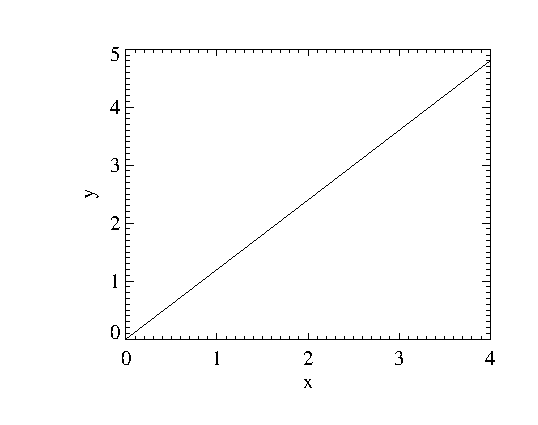
\includegraphics[width=3.75in]{simple.eps}
  \end{center}
  \caption{The figure caption made extra long so that the
    required spacing in the list of figures is evident.}
\label{fig:fig02}
\end{figure}
\lipsum[15]

\subsection{A Bit More Discussion}
\lipsum[16-19]


\endinput
%%
%% End of file `apxone.tex'.
